\documentclass[american,titlepage,oneside]{ntnuthesis}

\usepackage{parskip}
\setlength{\parskip}{10em}

\setlength{\marginparwidth}{2cm}
\usepackage{todonotes}

\title{Decentralized AI}
\shorttitle{Decentralized AI}
\author{Erik Dymbe}
\shortauthor{E. Dymbe}
\date{\today}

\addbibresource{thesis.bib}


% From https://www.overleaf.com/learn/latex/Glossaries

\makeglossaries % Prepare for adding glossary entries


\newglossaryentry{latex}
{
        name=latex,
        description={Is a mark up language specially suited for
scientific documents}
}

\newglossaryentry{bibliography}
{
        name=bibliography,
        plural=bibliographies,
        description={A list of the books referred to in a scholarly work,
typically printed as an appendix}
}

\newglossaryentry{maths}
{
    name=mathematics,
    description={Mathematics is what mathematicians do}
}


% --------------------
% ----- Acronyms -----
% --------------------

\newacronym{ai}{AI}{Artificial Intelligence}
\newacronym{als}{ALS}{Alternating Least Squares}
\newacronym{cf}{CF}{Collaborative Filtering}
\newacronym{dzai}{DzAI}{Decentralized Artificial Intelligence}
\newacronym{dzml}{DzML}{Decentralized Machine Learning}
\newacronym{dl}{DL}{Deep Learning}
\newacronym{fl}{FL}{Federated Learning}
\newacronym{gl}{GL}{Gossip Learning}
\newacronym{fm}{FM}{Factorization Machine}
\newacronym{ffm}{FFM}{Field-aware Factorization Machine}
\newacronym{gru}{GRU}{Gated Recurrent Unit}
\newacronym{hrnn}{HRNN}{Hierarchical Recurrent Neural Network}
\newacronym{lda}{LDA}{Linear Discriminant Analysis}
\newacronym{lr}{LR}{Logistic Regression}
\newacronym{ml}{ML}{Machine Learning}
\newacronym{mf}{MF}{Matrix Factorization}
\newacronym{mlp}{MLP}{Multilayer Perceptron}
\newacronym{nbc}{NBC}{Naive Bayes Classifier}
\newacronym{nn}{NN}{Neural Networks}
\newacronym{recsys}{RecSys}{Recommender System}
\newacronym{rnn}{RNN}{Recurrent Neural Network}
\newacronym{sgd}{SGD}{Stochastic Gradient Descent}
\newacronym{sl}{SL}{Supervised Learning}
\newacronym{svc}{SVC}{Support Vector Classifier}
\newacronym{ul}{UL}{Unsupervised Learning}
\newacronym{wma}{WMA}{Weighted Majority Algorithm} % add glossary and acronym lists before document

\begin{document}

\chapter*{Abstract}

Insert abstract here

\chapter*{Sammendrag}

Sett inn sammendrag her


\tableofcontents
\listoffigures
\listoftables
\lstlistoflistings

\printglossary[type=\acronymtype] % Print acronyms
\printglossary                    % Print glossary

\setlength{\parskip}{1em}

\chapter{Introduction}

\section{Motivation}

\section{Research Questions}
\subsection{How does decentralized learning methods compare to centralized solutions}
\chapter{Background and related work}
\label{chap:background}

\section{Deep Learning}

\section{Recommender systems}

\subsection{"Field-aware Factorization Machines for CTR Prediction", \citeyear{ffmctr} \cite{ffmctr}}

An effective method for classifying very large yet sparse data sets.

SOTA for several CTR-problems.

Has an over-fitting problem, but this can be mitigated by using early stopping.

\subsection{"Personalizing Session-based Recommendations with Hierarchical Recurrent Neural Networks", \citeyear{QuadranaKHC17} \cite{QuadranaKHC17}}

Simple matrix factorization does not take into account the timing and order of user events, and as a result are less responsiveness to changes in user behavior, e.g. new interests.

A \acrfull{rnn} can be used to exploit the timing and order of user events, but they may find it hard to model long sequences of user events over multiple sessions.

Because of this the \acrfull{hrnn} is introduced. It has two \acrfullpl{gru} instead of just one. One \acrshort{gru} models the session-level user activity, while another \acrshort{gru} models the user activity across sessions.

\subsection{"Temporal-Contextual Recommendation in Real-Time", \citeyear{tempcon} \cite{tempcon}}

2020. Introduces a black-box \acrshort{recsys} that can adapt to multiple use cases without the need for tuning. Achieves SOTA-performance on several data sets. Awarded best applied data science paper by SIGKDD for the 2020 digital conference.

Builds on the model described in \cite{QuadranaKHC17}, but improves on some aspects like efficiency, while still achieving comparable or even better results.

They also extended \acrshort{hrnn} by adding a \acrfull{ffm} that incorporates item and user features into the \acrshort{hrnn}. This new model is called \acrshort{hrnn}-meta.

\subsection{"Decentralized low-rank matrix completion", \citeyear{dezlowrank}, \cite{dezlowrank}}
\label{sec:dezlowrank}

Seems to give decent results compared to centralized methods, but it was not tested on any typical \acrshort{recsys} data set, so it's not clear if this method is viable yet.

Only tested for 50 agents, which is too low compared to a real scenario.

\subsection{"Decentralized Recommender Systems", \citeyear{WangLCZQH15} \cite{WangLCZQH15}}

Seems like a sketchy paper (collaborative \textbf{filleting}?), but some of them are supposedly connected to Samsung. 

Seems to be using the method used by \cite{dezlowrank}, although they give a simpler (but less detailed) explanation.

Testing on a pretty niche data set so not sure if their results are good or not, but their method is competitive.

Data only distributed across 8 agents, so not really a realistic scenario, the amount of agents should be in the thousands for this to be viable.

\subsection{"A Riemannian gossip approach to decentralized matrix completion", \citeyear{mishra2016riemannian}, \cite{mishra2016riemannian}}
\label{sec:mishra2016riemannian}

Probably the most viable decentralized matrix completion algorithm that I found.

Tested on the Netflix data set. Achieves decent results with a low amount of agents, however the performance decreases as the number of agents increase.

Maximum amount of agents that was tested was 20, so might not be competitive with thousands of users.

\subsection{"A Riemannian gossip approach to subspace learning on Grassmann manifold", \citeyear{mishra2018riemannian}, \cite{mishra2018riemannian}}
\label{sec:mishra2018riemannian}

Similar to the previous paper.

\subsection{"Decentralized and Privacy-Preserving Low-Rank Matrix Completion", \citeyear{Lin2015}, \cite{Lin2015}}
\label{sec:Lin2015}

Cited by \cite{mishra2018riemannian}. Does not benchmark on any recommender system data set, but it goes into detail as to how privacy preserving the approach is. Apparently it only provides weak privacy protection under a few assumption.

\begin{enumerate}
    \item The malicious agent is passive, i.e. it does not deviate from the optimization algorithm by provdiding any false values to any other agents. The paper argues that this is not unlikely as the agent might wants to avoid detection.
    \item The network topology is beneficial.
\end{enumerate}

\subsection{SVD}

"SVD++ has however some disadvantages, with the main drawback being that this method is not model-based. This means that if a new user is added, the algorithm is incapable of modeling it unless the whole model is retrained. Even though the system might have gathered some interactions for that new user, its latent factors are not available and therefore no recommendations can be computed. This is an example of a cold-start problem, that is the recommender cannot deal efficiently with new users or items and specific strategies should be put in place to handle this disadvantage."

\section{Centralized and decentralized \acrlong{mf}}

\subsection{Centralized}

In collaborative filtering the assumption is that users who give similar ratings will give similar ratings in the future as well. Another assumption is that a user will give similar ratings to similar movies.

Given a sparse user-movie ratings matrix a way to capture the aforementioned relationships is \acrfull{mf}. \acrshort{mf} decomposes the user-movie matrix into two matrices $W$ and $H$, see Figure \ref{fig:mf}. The H-matrix represents the latent features for each movie. The number of features is a hyperparameter that has to be tuned. Too few features will make it hard for the \acrshort{mf}-algorithm to fit the data well, but too many features will make the algorithm overfit the data. The features are learned during the decomposition of the original matrix. The $W$-matrix represents the preferences of each user towards each feature.

To find the predicted rating user $i$ will give to movie $j$, one can simply compute the dot product between row $i$  of $W$ and column $j$ of $H$.

A way to approximate $W$ and $H$ is to use gradient descent. The gradient for $h_{ij}$ depends on the values in column $j$ in the original user-movie matrix, column $j$ in H, as well as all values in $W$. The gradient for $w_{ij}$ depends on the values in row $i$ in the original user-movie matrix, row $i$ in W, as well as all values in $H$.

\begin{figure}
    \centering
    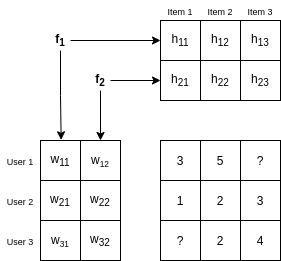
\includegraphics[width=0.5\textwidth]{figures/mf.png}
    \caption{Centralized Matrix Factorization}
    \label{fig:mf}
\end{figure}

\subsection{Decentralized}

In a decentralized context each agent can only access their own data, see Figure \ref{fig:d-mf}. The idea then is to collectively compute the $H$-matrix which is shared between all users, while each agents keeps their own local data as well as their own row of the $W$-matrix.

Given that the $H$-matrix is already computed, each agent has no problem computing $W$ on their own, as they have all the data needed to calculate gradients locally. The challenge is to collectively compute $H$ as each agent only has at most a single data point in the user-movie matrix that can be used to compute a gradient. This results in very noisy gradients. A possible solution could be to make the agents aggregate their gradients before applying them to $H$.

Multiple papers have done decentralized \acrlong{mf}, and although they vary slightly in the type of gradient descent they use, it seems like most used the public-private matrix method. See Section \ref{sec:dezlowrank} to Section \ref{sec:Lin2015} inclusively for these papers. Feel free to look them up. The math used in most of them is quite heavy though, so I have just been sticking to regular gradient descent for now. In my opinion the paper in Section \ref{sec:mishra2016riemannian} seemed pretty promising though.

\begin{figure}
    \centering
    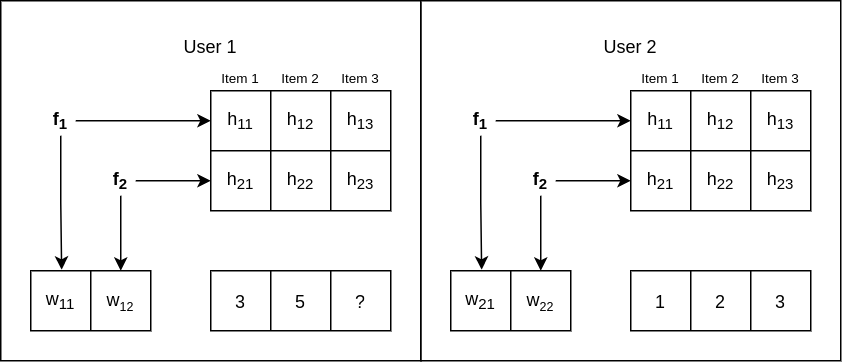
\includegraphics[width=\textwidth]{figures/d-mf.png}
    \caption{Decentralized Matrix Factorization}
    \label{fig:d-mf}
\end{figure}

\section{Decentralized Recommender Systems, \acrlong{fl} and \acrlong{gl}}

\subsection{"Federated Collaborative Filtering for Privacy-Preserving Personalized Recommendation System", \citeyear{ammaduddin2019federated}, \cite{ammaduddin2019federated}}

Introduces a \acrshort{fl}-approach to \acrshort{cf}. Argues that there is a need for a privacy-by-design solution for \acrlongpl{recsys} which does not store users data, while still making users data available for creating robust models. Uses \acrfull{als}. User vectors are calculated locally and not shared. The gradients for the item vector is also calculated locally, but are then aggregated on the central server. Formulated as an implicit feedback \acrshort{mf}-problem, although it is tested on Movielens, an explicit feedback dataset.

\subsection{"Meta Matrix Factorization for Federated Rating Predictions", \citeyear{lin2020meta}, \cite{lin2020meta}}

Uses \acrshort{fl} for users to train a \acrlong{nn} that does rating prediction. Meta-learning is used to create models that are smaller and better suited for mobile devices, the model on the central server is bigger than the models on the mobile devices. Has a central server, but none of the data is shared with the central server. Authors say that user information can be leaked through private item embeddings, RP
models and user updates.

\subsection{"Decentralized Recommendation based on Matrix Factorization: A Comparison of Gossip and Federated Learning", \citeyear{glrecsys}, \cite{glrecsys}}

Introduces a \acrshort{gl}-approach to recommendation systems. Uses \acrshort{sgd} instead of \acrshort{als} due to \acrshort{sgd} being more robust to failure and asynchrony. Vanilla \acrshort{gl} and vanilla \acrshort{fl} does not prevent the receiver of the gradients to try to calculate the users data, but there exists countermeasures for both approaches. Tries to model communication constraints and costs, while also testing the algorithm on the Movielens-dataset. \acrshort{gl} and \acrshort{fl} have similar performance. In general pretty low score on the Movielens-dataset, but this can be because of several reasons. First of all, the authors didn't use the most advanced models, due to it only being a comparison between the two decentralized algorithms. Another reason could be that the realistic modeling of communication restraints lowered performance.

\section{Decentralized Artificial Intelligence}
\subsection{Federated Learning}
\label{sec:federated-learning}

Traditional \acrfull{ml} approaches requires all of the data to be stored on a central machine, but there is a huge amount of data stored on edge devices that could be utilized for training useful \acrshort{ml} models. The owners of this data might not be willing to share it however.

This is why Google introduced \acrfull{fl} \cite{mcmahan2016communicationefficient}

\subsection{Gossip Learning}
\label{sec:federated-learning}

See \cite{gossiplearningalternative}

\subsection{Majority Voting}
\label{sec:mv}

\subsection{Weighted Majority Voting}
\label{sec:wmv}

TODO

\section{Related work}

\section{Market research}

Refer to previous paper?
\chapter{Centralized vs. decentralized learning}
\label{chap:general-dezai}

\section{Baseline for comparison}

To be able to compare decentralized methods to a centralized method a centralized baseline is needed. For simplicity, a fairly uncomplicated \acrfull{mlp} is chosen for this. See Figure \ref{fig:centralized-mlp} for the structure of the network. The strong model is trained for 5 epochs using \acrshort{sgd} on 12\,000 images sampled from the MNIST training dataset. Training the model 10 times with randomly initialized weights each time achieves an average accuracy of 93.71\% (0.16 \todo{clarify that this refers to percentage point?} standard deviation) on the whole MNIST test dataset consisting of 10\,000 images.

% np.mean(scores): 0.9370899999999999
% np.std(scores): 0.0016220049321749763

\begin{figure}
    \centering
    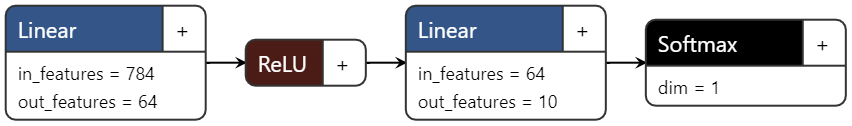
\includegraphics[width=\textwidth]{figures/simple-mlp.png}
    \caption{The architecture of a simple \acrshort{mlp}}
    \label{fig:centralized-mlp}
\end{figure} \todo{Explain dim=1 in Figure \ref{fig:centralized-mlp}?}

\section{Majority Voting}
\label{sec:mv-experiment}

\todo{Introduce majority voting earlier, and refer to it. Also: majority or plurality?}

An alternative to having one strong centralized model that produce a single prediction, is to use Majority Voting to aggregate the output from all the weak models into a single prediction.

To compare Majority Voting on multiple weak models to the baseline, a collection of models must be trained. Both the dataset, the \acrshort{mlp}-architecture, and the number of training epochs (see Figure \ref{fig:centralized-mlp}) must be the same as in the baseline experiment to make the comparison fair. With 12\,000 data points in the training dataset, and if each weak model got 32 data points each, a total of 375 models are trained.

Training each model for 5 epochs on a training dataset of 32 data points achieves an average accuracy of 25.23\% (0.27 standard deviation) when repeating this 10 times on the whole MNIST test dataset. This is indeed a very weak model, especially considering an accuracy of 10\% can be achieved by blindly guessing. This is however to be expected with such a small training dataset. Considering the MNIST classification task has 10 different output classes, each individual model will only have approximately 3 data points for each class.

This accuracy is dramatically improved upon by using Majority Voting. Using Majority Voting to aggregate the 375 outputs into a single prediction for each data point in the test dataset yields an accuracy of 72.52\% (1.27 standard deviation) when running 10 times with randomly initialized models. See Figure \ref{fig:example-votes} for the result of two example votes. This is a dramatic improvement in accuracy compared to the accuracy of each individual model. The accuracy is however still significantly lower than the baseline model. It is also worth noting that the Majority Voting method has to calculate the output of all the 375 models and then aggregate it, while the baseline method only has to calculate the output of a single model. Majority voting might therefore be unsuited for applications where speed or resource use is critical.

\begin{figure}
    \begin{subfigure}{.5\textwidth}
        \centering
        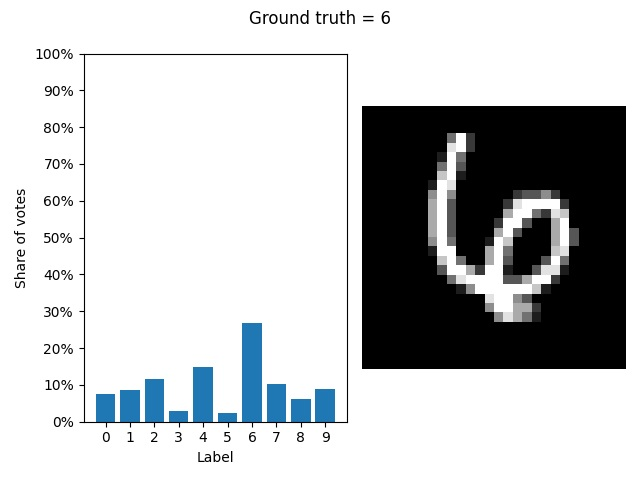
\includegraphics[width=\linewidth]{figures/example-vote-1.jpg}
        \caption{}
        \label{fig:example-votes-a}
    \end{subfigure}
    \begin{subfigure}{.5\textwidth}
        \centering
        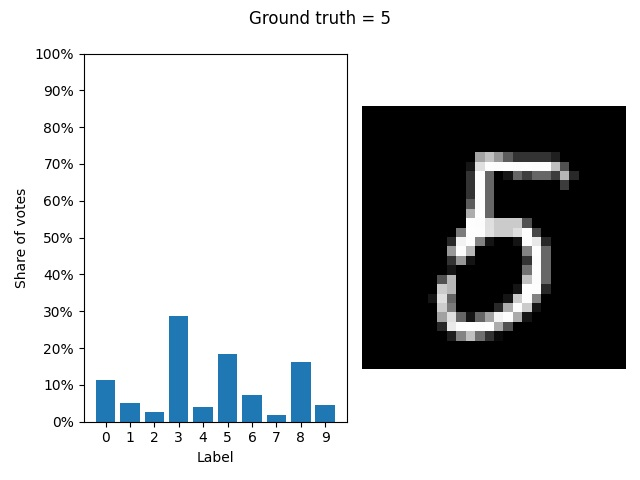
\includegraphics[width=\linewidth]{figures/example-vote-2.jpg}
        \caption{}
        \label{fig:example-votes-b}
    \end{subfigure}
    \caption{Two example voting results when the 375 models vote for which label to assign each image. On Figure \ref{fig:example-votes-a} the image was correctly classified as a six due to that label receiving the highest share of the votes, while on Figure \ref{fig:example-votes-b} the image was incorrectly classified as a three due to that label receiving the highest share of the votes.}
    \label{fig:example-votes}
\end{figure}

\section{Model aggregation}

Calculating the output of every model to do majority voting can be very inefficient. A more efficient method is to aggregate all the models to produce a single model. One way of producing an aggregated \acrshort{mlp} is to set its weights and biases to the means of all of the models weights and biases. This works as long as all of the aggregated models were initialized with the same values. To test this 375 models were trained in the same way as in Section \ref{sec:mv-experiment}, only this time they were all given the same initialization. An aggregated model is then produced by averaging their parameters.

This experiment is run 10 times. Looking at the output from individual tests one can immediately see that there is a similarity between the average output for all models and the output of the aggregated model. See Figure \ref{fig:aggr-vs-mean} for two examples of this. The average accuracy for the aggregated model is 32.98\% (2.94 standard deviation) for all of the 10 runs. This is an improvement to the average accuracy of the individual models, which was 26.44\% (1.44 standard deviation). This is still less than the average accuracy achieved by Majority Voting, which is 36.51\% (4.17 standard deviation). Interestingly the accuracy of the Majority Vote was significantly worse in this experiment compared to the experiment in Section \ref{sec:mv-experiment}, where all of the models are initialized with different weights and biases, as opposed to this experiment were all of the models were initialized with the same weights and biases.

\begin{figure}
    \begin{subfigure}{.5\textwidth}
        \centering
        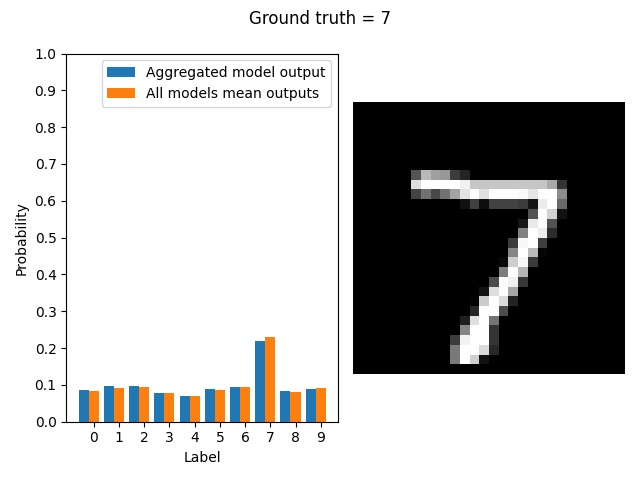
\includegraphics[width=\linewidth]{figures/aggr-vs-mean-1.jpg}
        \caption{}
        \label{fig:aggr-vs-mean-a}
    \end{subfigure}
    \begin{subfigure}{.5\textwidth}
        \centering
        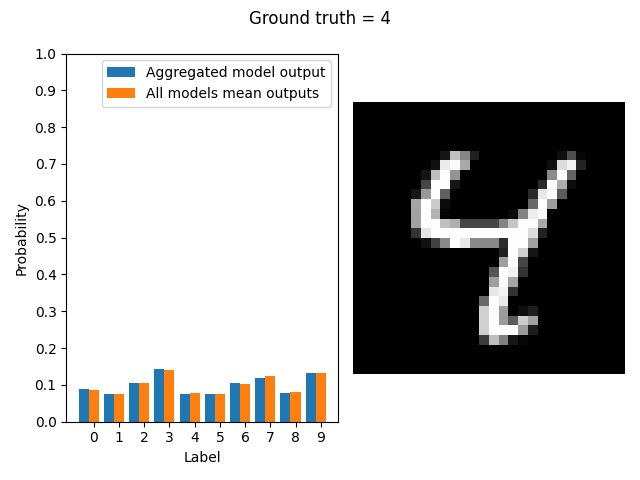
\includegraphics[width=\linewidth]{figures/aggr-vs-mean-2.jpg}
        \caption{}
        \label{fig:aggr-vs-mean-b}
    \end{subfigure}
    \caption{Two examples of the output from a model aggregated from 375 models (in blue) drawn together with the mean output of those 375 models (in orange). Note that the aggregated model has a very similar output to the mean output of the models it is aggregated from.}
    \label{fig:example-votes}
\end{figure} \label{fig:aggr-vs-mean}

\section{Weighted Majority Voting}
\label{sec:wmv-experiment}

Some models might be more accurate than others, Majority Voting might therefore not be the best choice as it weights all the models predictions equally. Weighted Majority Voting (see Section \ref{sec:wmv} might therefore be a better alternative. For testing this method, the exact same models are used as in Section \ref{sec:wmv-experiment}, but when evaluating Weighted Majority Voting the weight for each models prediction is adjusted if they they were wrong on the previous input (see Section \ref{sec:wmv}).

After 10 runs with randomly initialized models, surprisingly the Weighted Majority Voting method produced worse results than Majority Voting. With $\beta=0.05$ Weighted Majority achieved an average accuracy of 44.40\% (1.16 standard deviation) over 10 runs, which is less than what Majority Voting scored in Section \ref{sec:mv-experiment}. Weighted Majority Voting consistently scored lower for all values of $\beta$ that was tested, except for $\beta = 0$ which is in essentially exactly the same as using Majority Voting as the weights will be the same for every iteration. A higher $\beta$-value seemed to only make the accuracy of the Weighted Majority converge to the accuracy of its most accurate expert faster. See Figure \ref{fig:wmv-over-time-beta} for an example of this.

\begin{figure}
    \begin{subfigure}{.5\textwidth}
        \centering
        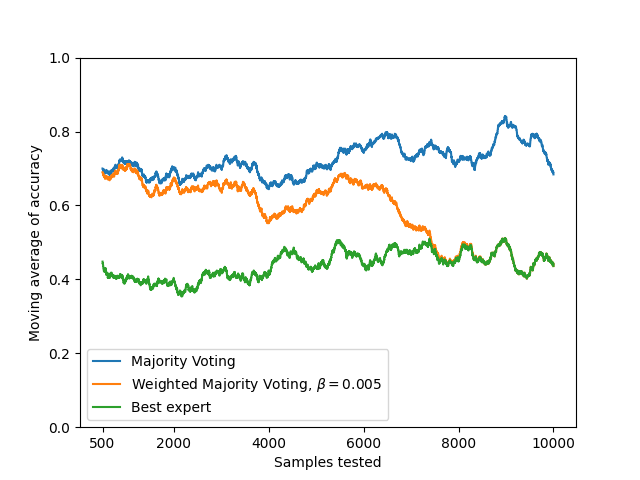
\includegraphics[width=\linewidth]{figures/wmv-beta0_005.png}
        \caption{}
        \label{fig:wmv-over-time-beta-a}
    \end{subfigure}
    \begin{subfigure}{.5\textwidth}
        \centering
        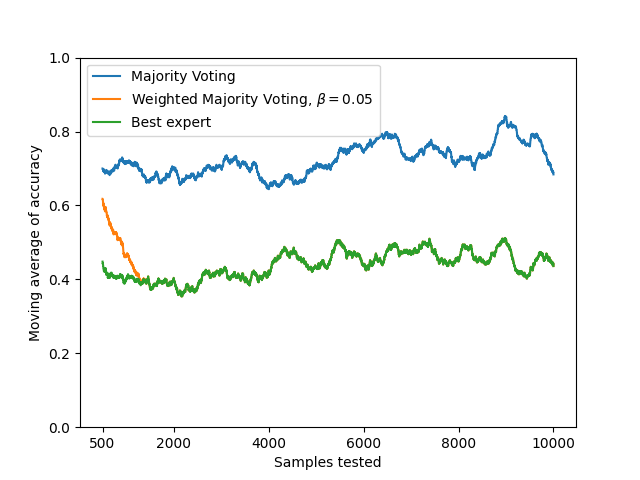
\includegraphics[width=\linewidth]{figures/wmv-beta0_05.png}
        \caption{}
        \label{fig:wmv-over-time-beta-b}
    \end{subfigure}
    \caption{The moving average of the accuracy of the the result from the Majority Vote, Weighted Majority Vote, and the best model. Plotted in blue, orange and green respectively. The moving average has a width of 500 samples, which is why the graph starts at sample 500. Notice how the accuracy of the Weighted Majority Vote start out with a similar accuracy as the Majority Votes as most of the experts have similar weights in the beginning, but over time the accuracy starts to converge to the accuracy of its best expert. Notice that the accuracy of Weighted Majority Voting converged slower on Figure \ref{fig:wmv-over-time-beta-a} than on Figure \ref{fig:wmv-over-time-beta-b} due to it having a lower $\beta$-value.}
    \label{fig:example-votes}
\end{figure} \label{fig:wmv-over-time-beta}

Over time, the best expert will dominate the rest of the experts if it continues being the best. An example of this can be seen on Figure \ref{fig:mv-vs-wvm-vote}. This might be desirable in situations where one expects that one expert is significantly more accurate than the other experts, but in this experiment both the testing and training data is uniformly sampled, which means that any advantage any expert has is just a result of a lucky sampling of the training data for that expert. And since the distribution of the test data does not change over time it is likely that the best expert will continue to dominate the other experts for the rest of the experiment. If the test distribution changes over time Weighted Majority Voting could perhaps have an advantage over Majority Voting since it could use the best expert for each different test distribution. This would however also require that some experts were significantly better than the rest of the experts at specific distributions, which could be the case if their training data was sampled from different distributions.

\begin{figure}
    \begin{subfigure}{.5\textwidth}
        \centering
        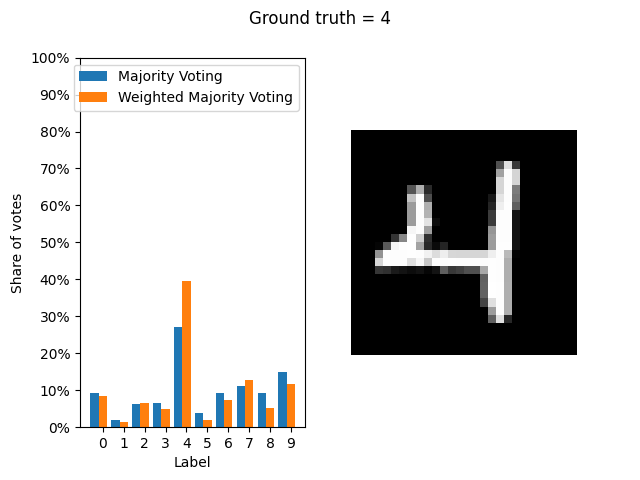
\includegraphics[width=\linewidth]{figures/mv-vs-wmv-1.png}
        \caption{}
        \label{fig:mv-vs-wvm-vote-a}
    \end{subfigure}
    \begin{subfigure}{.5\textwidth}
        \centering
        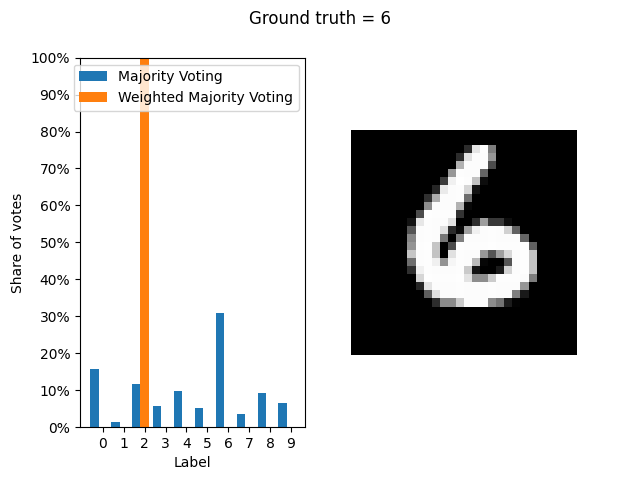
\includegraphics[width=\linewidth]{figures/mv-vs-wmv-2.png}
        \caption{}
        \label{fig:mv-vs-wvm-vote-b}
    \end{subfigure}
    \caption{The distribution of votes for Majority Voting and Weighted Majority Voting. Figure \ref{fig:mv-vs-wvm-vote-a} shows a voting result fairly early in the testing process. Some experts are therefore weighted heavier than others, but no single expert dominates the vote yet. Figure \ref{fig:mv-vs-wvm-vote-b} shows the voting result fairly late in the testing process. At this stage the weights of the other experts are so low in comparison to the most accurate expert that their votes are effectively ignored. A single expert dominates.}
\end{figure} \label{fig:mv-vs-wvm-vote}

% TODO: Majority voting glossary?

\section{Remove class-bias}
\label{sec:reduce-bias}

In section \ref{sec:wmv-experiment} using Majority Voting seemed to in general yield better results than any single expert. A possible explanation for why could be that the Majority Voting method reduces the bias of all the experts by averaging it out\todo{this needs an explanation or a proof}. The source for the bias of the experts is the different training data that they are trained on. A hypothesis is that the best expert may be better than the Majority Vote if all of the experts are unbiased, since the bias-reduction properties of Majority Voting will then be redundant. In the previous experiments all of the experts where trained on 32 data points sampled randomly without replacement from the training dataset. This means that each expert have a different amount of data points coming from each class. In fact, since there's 10 classes, and the experts only get 32 data points each, it is impossible for an expert to have the same amount of data points from each class. Each expert therefore have a certain bias towards one or more classes.

To reduce the class bias one can make sure each expert receives the same amount of data points from each class. For this to be possible the training set of each expert has to be a multiple of the amount of classes, which is in the case of the MNIST-problem is 10. Instead of each expert having 32 data points in their training set they will therefore only have 30 in the following experiment. Each expert will randomly sample 3 data points from each class. See Figure \ref{fig:bias} for a run without and a run with class-bias reduction.

\begin{figure}
    \begin{subfigure}{.5\textwidth}
        \centering
        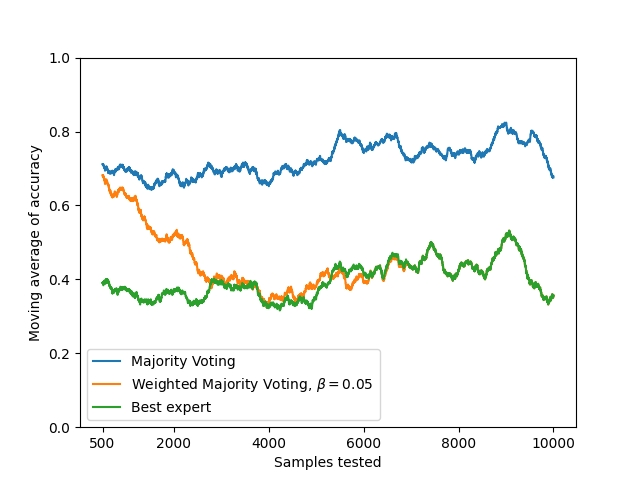
\includegraphics[width=\linewidth]{figures/bias-1.jpg}
        \caption{}
        \label{fig:bias-a}
    \end{subfigure}
    \begin{subfigure}{.5\textwidth}
        \centering
        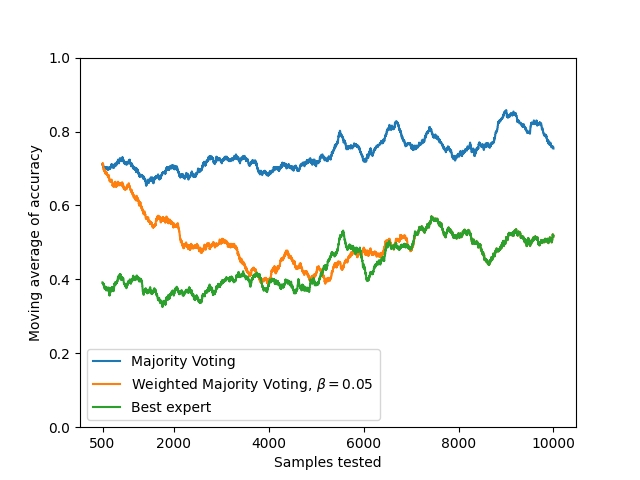
\includegraphics[width=\linewidth]{figures/bias-2.jpg}
        \caption{}
        \label{fig:bias-b}
    \end{subfigure}
    \caption{The moving average of the accuracy when using Majority Vote, Weighted Majority Vote, and the best expert. Plotted in blue, orange and green respectively. The moving average has a width of 500 samples, which is why the graph starts at sample 500. On Figure \ref{fig:bias-a} each expert is trained on 30 data points not necessarily evenly distributed across the 10 classes, while on Figure \ref{fig:bias-b} the 30 data points are evenly distributed, meaning each class is guaranteed 3 data points.}
    \label{fig:example-votes}
\end{figure} \label{fig:bias}

From the result from the experiment it is not clear whether or not reducing the class-bias made the Weighted Majority Vote converge faster or slower to the best expert. But it is clear that the Majority Vote still outperforms the best expert even when class-bias is taken into account. A possible explanation for this could be that there are more types of bias than class-bias. This could for example be a bias towards certain features.

It is however clear that removing class-bias slightly improves the performance of the individual experts. After 10 runs with random initialization the average accuracy of the experts was 25.15\% (0.33 standard deviation) without removing the class-bias, but 27.72\% (0.29 standard deviation) when removing the class-bias. This also leads to the Majority Vote performing better. Without removing class-bias the Majority Vote has an average accuracy of 72.59\% (1.19 standard deviation), while when removing the class-bias an average accuracy of 75.71\% (1.27 standard deviation) was achieved.

Reducing the class-bias might in a lot of scenarios not be possible. For a lot of problems the real class distribution might not be known. Also, in a decentralized context, the control of the data used to train each expert might be limited.

\section{Non-static test distribution}

In previous experiments the test data was drawn from the same distribution throughout the whole experiment. I could be of interest to see if Weighted Majority Voting would outperform Majority Voting if the test distribution changed over time. In the previous experiments the performance of Weighed Majority Voting always converged to the performance of the most accurate expert. If the the test distribution changes over time, then it is possible that the best expert might change over time as well, as some experts might be better at some distribution than others.

This hypothesis was tested by running both Majority Voting and Weighted Majority Voting on a segmented test set. Each segment of the test set being biased towards a specific digit, starting at 0 and ending at 9. On Figure \ref{fig:biased-test-a} each segment contains 50\% of the data it is biased towards, while on \ref{fig:biased-test-b} each segment only contain the data it is biased towards.

\begin{figure}
    \begin{subfigure}{.5\textwidth}
        \centering
        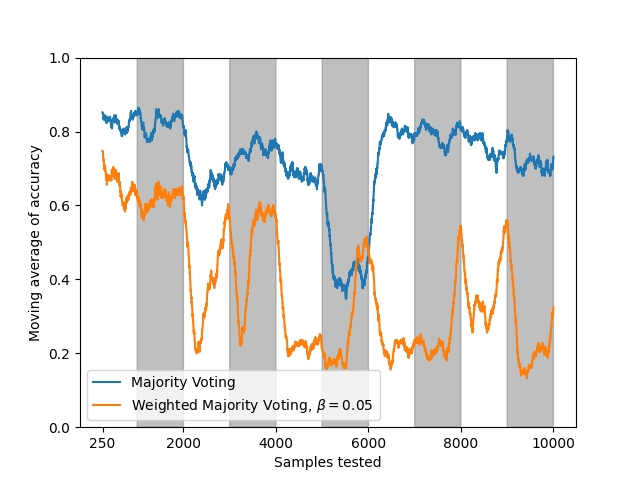
\includegraphics[width=\linewidth]{figures/biased-test-1.jpg}
        \caption{}
        \label{fig:biased-test-a}
    \end{subfigure}
    \begin{subfigure}{.5\textwidth}
        \centering
        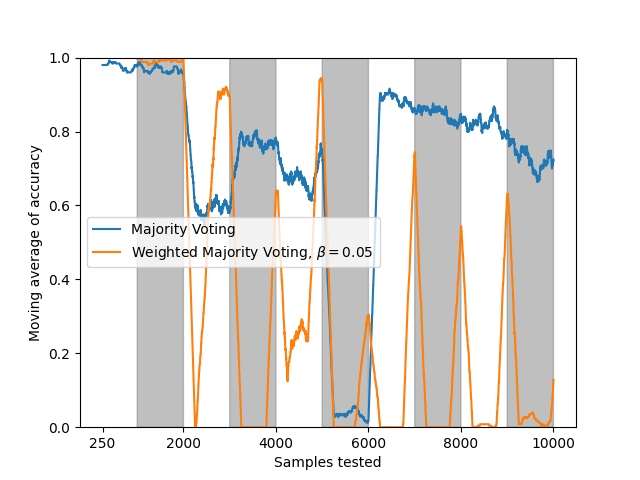
\includegraphics[width=\linewidth]{figures/biased-test-2.jpg}
        \caption{}
        \label{fig:biased-test-b}
    \end{subfigure}
    \caption{The moving average of the accuracy when using Majority Vote and Weighted Majority Vote, plotted in blue, and orange respectively, for biased test distributions. On Figure The moving average has a width of 250 samples, which is why the graph starts at sample 250.}
\end{figure} \label{fig:biased-test}

Even with a changing distribution during the experiment, Weighted Majority Voting was still unable to consistently outperform Majority Voting. Weighted Majority Voting was able to outperform Majority Voting a few times, especially in the second experiment as can be seen in Figure \ref{fig:biased-test-b}, but this was always only for a short duration, and it was invariably followed by a significant crash in performance as soon as the distribution changed. This was because the experts that got weighed heavier for each segment were usually the experts that were heavily biased towards the biased digit of that segment. Some of these experts simply predicted the same digit for almost every input.

\section{Using a classifier on expert predictions}

Neither Majority Voting or Weighted Majority Voting managed to come close to the performance of the baseline expert. New ways of aggregating the results should therefore be explored. One possible way of doing this is to phrase it as a \acrshort{sl} problem. \todo{Can I call the involved parties experts, or does that term refer to the model?} Each involved party in a \acrshort{dzai} context has their own local data. They can also receive models from other parties. This means that they can generate feature vectors from the predictions made by the models on their local data. This together with the true label can be used to train a classifier.

One problem with this approach is that the output of data put through a model that was trained on the same data can not be used as features vectors. This is because these outputs would seem much more accurate than they actually are, a classifier would therefore incorrectly assume that this output is way more accurate than they really are. Another challenge is that each party only has a limited amount of training data. In previous experiments each expert was trained on only 30 data points. It would therefore be fair to assume that each party only have 30 data points in this experiment as well. That is not a lot of data for training a classifier with a high dimensional input space. If there are 399 other parties like in the previous experiments, then the input space would be 399-dimensional if the numerical outputs of each expert is used, and 3990 if one-hot-encoding is used.

For this experiment four different classifiers are used. A \acrfull{svc}, a \acrfull{nbc}, \acrfull{lda}, and \acrfull{lr}. Each classifier is trained on 30 data points, each data points consisting of the output of 399 experts. Each classifier is then tested on the MNIST test set. This experiment is repeated ten times with randomly initialized and trained experts. See Table \ref{tab:4-classifiers} for the result.

\begin{table}[]
    \centering
    \begin{tabular}{|c|c|}\hline
        Classifier      & Accuracy (STD) \\\hline
        \acrshort{svc}  & 46.54\% (0.60) \\
        \acrshort{nbc}  & 45.34\% (1.24) \\
        \acrshort{lda}  & 39.28\% (1.10) \\
        \acrshort{lr}   & 56.46\% (0.75) \\\hline
    \end{tabular}
    \caption{The accuracy averaged over ten runs for each type of classifier with the standard deviation in parenthesis}
    \label{tab:4-classifiers}
\end{table}

As can be seen on Table \ref{tab:4-classifiers} for the result, none of the classifiers managed to outperform a simple Majority Vote when they were only trained on 30 data points. Considering the high dimensionality of the input vector this is to be expected.

A possible solution for this lack of data could be to have parties share generated feature vectors. \todo{The security of this is questionable. Can the private data not be reconstructed in any way?} This way they do not directly share their own private data. They do however have to share the true label of these feature vectors, which could be a privacy breach in some scenarios.

See Figure \ref{fig:acc-vs-data-clfs} to see how the accuracy increases as more data is added.

\begin{figure}
    \centering
    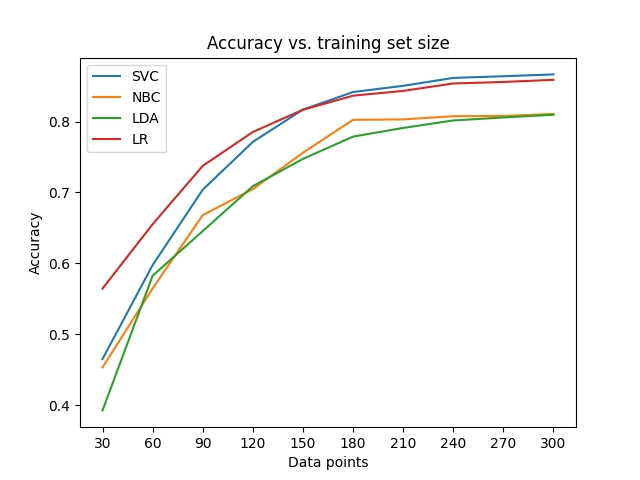
\includegraphics[width=0.9\linewidth]{figures/acc-vs-data-clfs.jpg}
    \caption{Caption}
    \label{fig:acc-vs-data-clfs}
\end{figure}
\chapter{Semi-decentralized recommendation system}
\label{chap:discussion}

Possibilities:

\section{Aggregate gradients on agent trusted by multiple agents}


\input{chapters/5-discussion.tex}

\chapter*{\bibname}
\printbibliography[heading=none]

% First paper

%\begin{paper}{papers/landes1951scrutiny.pdf}{paper:scrutiny}
%    Here, you may add a description of the paper, an illustration, or just give the bibliographic reference:
%    \begin{quote}
%        \fullcite{landes1951scrutiny}
%    \end{quote}
%    Or you may leave it empty, if you like.
%\end{paper}

% Second paper etc.

\appendix
\input{appendices/a-appendix.tex}

\end{document}
